\subsubsection{hypre} 


\paragraph{Overview} 
The {\sl hypre} software library \cite{hypre,hypre_design_impl_2006} provides high performance preconditioners and solvers for the solution of large sparse linear systems on massively parallel computers, with particular focus on algebraic multigrid solvers. One of {\sl hypre}’s unique features is the provision of a (semi)-structured interface, in addition to a traditional linear-algebra based interface. The semi-structured interface is appropriate for applications whose grids are mostly structured, but with some unstructured features. Examples include block-structured grids, composite grids in structured adaptive mesh refinement (AMR) applications, and overset grids. These interfaces give application users a more natural means for describing their linear systems, and provide access to methods such as structured multigrid solvers, which can take advantage of the additional information beyond just the matrix. Since current architecture trends are favoring regular compute patterns to achieve high performance, the ability to express structure has become much more important. The {\sl hypre} library provides both unstructured and structured multigrid solvers, which have shown excellent scalability on a variety of high performance computers, e.g Blue Gene systems (unstructured solver BoomerAMG has scaled up to 1.25 million MPI cores with a total of 4.5 million hardware threads). It is used by many ECP application teams, including ExaAM, Subsurface, ExaWind, CEED, and more. It requires a C compiler and an MPI implementation, but it also runs in an OpenMP environment. It has some GPU capabilities.
\paragraph{Key  Challenges}

While {\sl hypre}'s solvers contain much parallelism, their main focus is the solution of sparse linear systems, leading to  very large demands on memory bandwidth. In addition, the use of multiple levels, while greatly aiding convergence of the solvers, leads to decreasing systems sizes, number of operations and parallel efficiencies on coarser levels. Particularly the unstructured algebraic multigrid solver BoomerAMG\cite{HeYa2002}, which is {\sl hypre}'s most often used preconditioner, suffers from increasing communication complexities on coarser levels. Coarse grid operators are generated by multiplying three matrices leading to increasing numbers of nonzeroes per row in the resulting matrices and with it increasing numbers of neighbor processes. While BoomerAMG's solve phase mainly consists of matrix vector products and smoothing operations, which are fairly straight forward to parallelize, even on a GPU, its setup phase is highly complex, including many branches, a lot of integer operations as well as some sequential passages. Current  interpolation strategies that lead to best convergence and performance on distributed memory machines are not suitable for implementation on GPUs or similar architectures requiring extreme parallelism. There are several algorithms that are more suitable for GPUs, such as direct interpolation, which however leads to degraded convergence. It could possibly be improved using Jacobi interpolation. All these options would need to be implemented and tested on GPUs. Since {\sl hypre} is a mature product with many solvers and interdependent features, any significant changes that affect the whole library, are tedious and require much testing to ensure that the library stays backward compatible and no features are broken.

\paragraph{Solution Strategy}

Since the upcoming computer architectures are heterogeneous with accelerators, it was very important to enable {\sl hypre} for GPUs. We looked into various options, such as the use of CUDA, OpenMP 4.5, as well as RAJA and Kokkos. We limited the latter two options to the structured interface and solvers which are more natural candidates for such an approach due to their use of macros, called BoxLoops, for loops.
Since computer architectures continue to change rapidly, it is important to come up with strategies that will facilitate future porting of the software. Therefore we decided to develop a new memory model that addresses the use of different memory locations.

\paragraph{Recent Progress}

Under internal LLNL funding we pursued the following ECP-related tasks: enabling portions of several solvers for GPUs, and introducing a new memory model that is based on an abstract machine model.

We  implemented the new memory model. The new model modified {\sl hypre}'s memory allocation and copying routines to include memory allocations: HYPRE$\_$MEMORY$\_$HOST, HYPRE$\_$MEMORY$\_$DEVICE and HYPRE$\_$MEMORY$\_$SHARED. It also includes a new routine SetExecutionMode that can be used to define where the current code can be run.
The new model can be mapped to the actual hardware in a variety of ways through the configure process, e.g., a host-only machine (all allocations are just mallocs) or with or without unified memory. Since it is based on an abstract machine model, it is expected that it will increase portability to future architectures. The implementation of the model was very intensive, since it affected the whole library. 

In addition, we implemented various GPU capabilities in {\sl hypre}. For the structured solvers, SMG and PFMG\cite{AsFa1996}, both setup and solve phase can now completely be run on GPUs, using both CUDA or OpenMP4.5, and do not require unified memory. In addition, options to use RAJA and Kokkos are available, albeit not well tested yet. Figure \ref{fig:pfmg} shows the performance of the total run times, including both setup and solve phase, for our fastest performing multigrid solver PFMG-CG for a 7-point 3D Laplace problem using 32 million grid points per node, comparing performance on the CPU only utilizing all its cores, to running the same problem on the GPUs using CUDA and OpenMP 4.5.

\begin{figure}
\centering
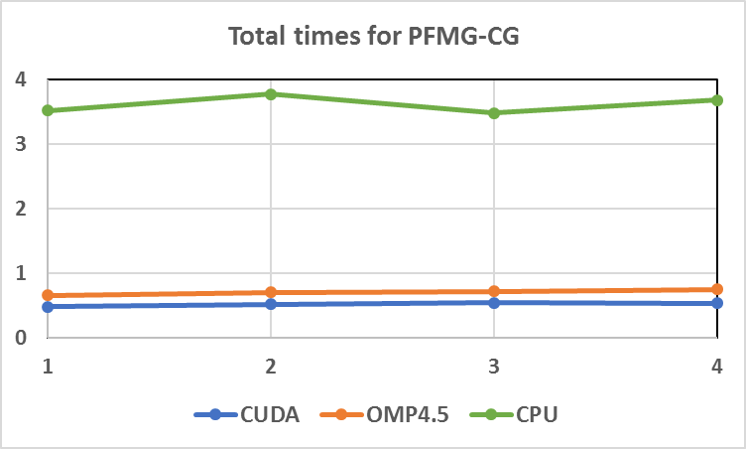
\includegraphics[width=5in]{projects/2.3.3-MathLibs/2.3.3.01-xSDK/PFMG-PCG.png}
\caption{\label{fig:pfmg} Performance of PFMG-PCG on Ray at LLNL, using Power 8 CPUs and Pascal GPUs}
\end{figure}

Porting the unstructured solver, BoomerAMG turned out to be far more complex. Currently only the solve phase can be run on the GPU for select smoothers, mainly Jacobi smoothers, and requires unified memory. The setup phase can currently be performed on the CPU only.


\paragraph{Next Steps}

Our most immediate plans are to improve the efficiency of interfacing applications with {\sl hypre}'s solvers. This includes removal of unnecessary copies, and increasing use of threading, wherever possible. We plan to remove the requirement to use unified memory for BoomerAMG and want to increase the portions of its solve phase that are not GPU-enabled yet, but are well suited for GPUs, e.g. polynomial smoothers. Further out we would like to investigate how to enable the setup phase for GPUs, initially porting algorithms that are suitable as well as finding ways to improve convergence where necessary.
In addition, we would like to work with ECP application teams who are using {\sl hypre} or would like to use it, to achieve best performance by tuning the solvers for them and potentially implementing suitable algorithmic changes. One example would be the implementation of ICGS-GMRES to improve ExaWind's solve times.

Other interesting topics that could impact ECP applications, but are currently pursued under SciDAC funding is the development of parallel smoothers that lead to better convergence than Jacobi, such as ILU related methods, as well as the development of multigrid solvers that are more capable to take advantage of the structure of a problem.

